\documentclass[a4paper,11pt,UTF8]{afthesis}
\usepackage{ctex}
\usepackage{amsmath,amsthm,amssymb,amsfonts}
\usepackage{amsmath}
\usepackage[a4paper]{geometry}
\usepackage{graphicx}
\usepackage{microtype}
\usepackage{siunitx}
\usepackage{booktabs}
\usepackage[colorlinks=false, pdfborder={0 0 0}]{hyperref}
\usepackage{cleveref}
\usepackage{esint} 
\usepackage{graphicx}
\usepackage{ragged2e}
\usepackage{pifont}
\usepackage{extarrows}
\usepackage{mathptmx}
\usepackage{float}
\usepackage{caption}
\usepackage{subfigure}

\captionsetup[figure]{name={Figure}}

\title{Microelectronics Circuit Analysis and Design Homework(15th)}
\author{Yuejin Xie \quad U202210333}
\date{Nov 15th, 2023}
\begin{document}
\maketitle
15.15 Consider the bandpass filter in Figure P15.15.(a) Show that the voltage transfer function is
$$
A_v(s)=\frac{v_O}{v_I}=\frac{-1/R_4}{(1/R_1)+sC+1/(sCR_2R_3)}
$$
(b) For $C= 0.1\mu$F, $R_1=85$ k$\Omega,\quad R_2=R_3=300\Omega,\quad R_4=3$ k$\Omega$, and
$R_5=30$ k$\Omega$, determine: (i) $|A_v( $max$) |; $(ii) the frequency $f_o$ at which $|A_v( $max$) |$ occurs; and (iii) the two 3 dB frequencies.


\begin{figure}[H]
	\centering
	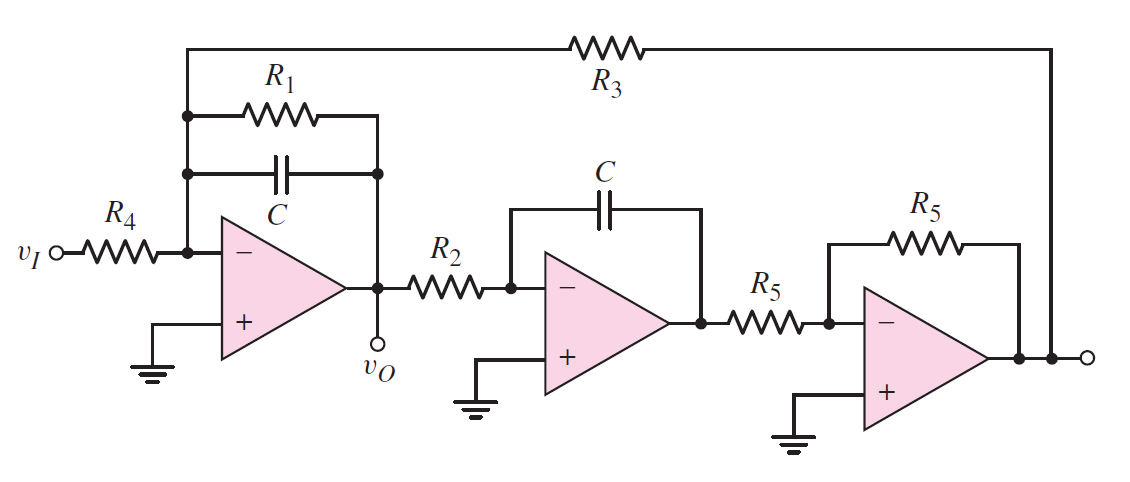
\includegraphics[width=0.6\textwidth]{15.15}
	\caption{Problem 15.15}
\end{figure}
\noindent Solution:

(a)Because of "KCL", and virtual open and short, we have equation as follow:

$$\left\{\begin{aligned}
	&\frac{v_I}{R_4} =-\frac{v_{2}}{R_{3}}-\frac{v_{o}}{R_{1}\left\|\left(\frac{1}{sC}\right)\right.}  \\
	&\frac{v_o}{R_2} =-\frac{v_{1}}{\left(\frac1{sC}\right)}  \\
	&\frac{v_{1}}{R_{5}} =-\frac{v_{2}}{R_{5}} 
\end{aligned}\right.\Rightarrow A_v(s)=\frac{v_O}{v_I}=\frac{-1/R_4}{(1/R_1)+sC+1/(sCR_2R_3)}$$

(b)$C= 0.1\mu$F, $R_1=85$ k$\Omega,\quad R_2=R_3=300\Omega,\quad R_4=3$ k$\Omega$, and
$R_5=30$ k$\Omega$, Now
$$\begin{aligned}
	A_v(s)&=\frac{v_O}{v_I}=\frac{-1/R_4}{(1/R_1)+sC+1/(sCR_2R_3)}=-\frac{R_1}{R_4}\cdot\frac{1}{1+sR_1C+\dfrac{R_1}{sCR_2R_3}}\\
	&=-\frac{R_1}{R_4}\cdot\frac{1}{1+j(\omega R_1C-\dfrac{R_1}{\omega CR_2R_3})}
\end{aligned}\\
$$
$$
	 \begin{aligned}\Rightarrow\left|A_{V}(j\omega)\right|=\frac{R_{1}}{R_{4}}\cdot\frac{1}{\sqrt{1+(\omega R_1C-\dfrac{R_1}{\omega CR_2R_3})^2}}\end{aligned}
$$

(i)When $\omega R_1C-\dfrac{R_1}{\omega CR_2R_3}=0, |A_v(jw)|_{\max}=28.33$

(ii)$\omega =\dfrac{1}{C\sqrt{R_1R_2}}, f_o=\dfrac{\omega}{2\pi}=5.31\mathrm{kHz}$

(iii)For 3dB frequencies, we have equation:
$$(\omega R_1C-\dfrac{R_1}{\omega CR_2R_3})^2=1, f=\frac{\omega}{2\pi}\Rightarrow f= 5.32 \mathrm{kHz}, 5.30 \mathrm{kHz}$$
15.17 For each of the circuits in Figures P15.17, derive the expressions for the voltage transfer function $T(s)=V_o(s)/V_i(s)$ and the cutoff frequency $f_{3\text{dB}}.$
\begin{figure}[H]
	\subfigure[]{
		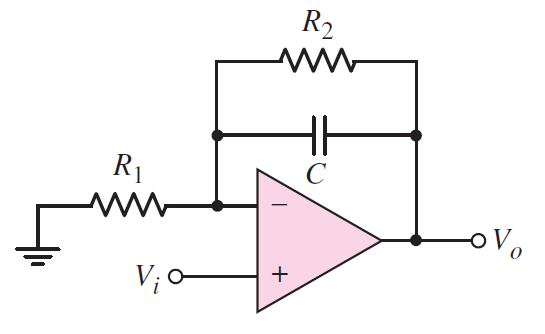
\includegraphics[width=0.4\textwidth]{15.17_a}
	}
	\subfigure[]{
		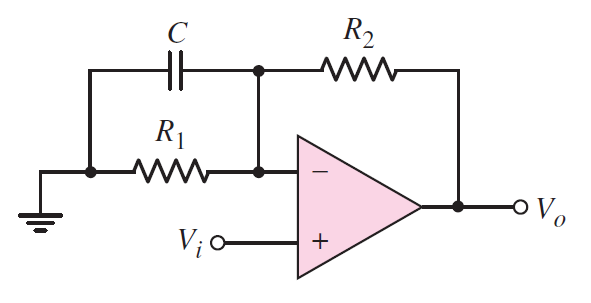
\includegraphics[width=0.4\textwidth]{15.17_b}
	}
	\centering

	\caption{Problem 15.17}
\end{figure}
\noindent Solution:

(a)Because of "KVL", and virtual open and short, we have equation:
$$
	T(s)=V_o(s)/V_i(s)=\frac{R_1+R_2||\frac1{sC}}{R_1}=\left(1+\frac{R_{2}}{R_{1}}\right)\cdot\frac{1+s(R_{1}\parallel R_{2})C}{1+sR_{2}C}
$$
$$
	\Rightarrow f_H=\frac{1}{2\pi R_2C}, f_L=\frac{1}{2\pi (R_1||R_2)C}
$$
(b)Because of "KVL", and virtual open and short, we have equation:
$$
\Rightarrow T(s)=V_o(s)/V_i(s)=\frac{R_2+R_1||\frac1{sC}}{R_1||\frac1{sC}}=\frac{R_{2}+R_{1}}{R_{1}}\cdot\left(1+s(R_{1}\parallel R_{2})C\right)
$$
$$
	\Rightarrow f=\frac{1}{2\pi (R_1||R_2)C}
$$

15.46 Consider the Schmitt trigger in Figure P15.46. Assume the saturated output voltages are $\pm V_P.$ (a) Derive the expression for the crossover voltages $V_{TH}$ and $V_{TL}$. (b) Let $R_A=10$ k$\Omega$, $R_B=20$ k$\Omega,\:R_1=5$ k$\Omega,\:R_2=20$ k$\Omega$, $V_P=10$ V, and $V_{\mathrm{REF}}=2$ V. (i) Find $V_{TH}$ and $V_{TL}$. (ii) Sketch the voltage transfer characteristics.
\begin{figure}[H]
	\centering
	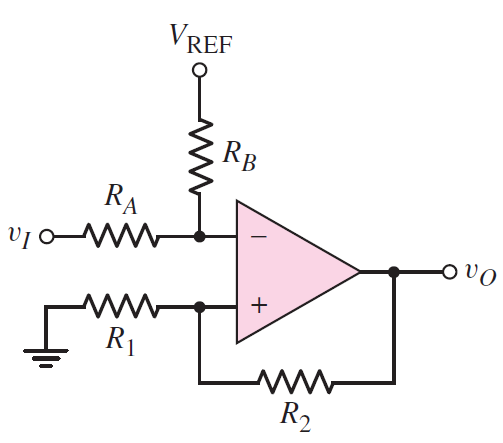
\includegraphics[width=0.4\textwidth]{15.46}
	\caption{Problem 15.46}
\end{figure}
\noindent Solution:

(a)For $V_O=+V_P$:
$$
\frac{R_A}{R_A+R_B}V_{REF}+\frac{R_B}{R_A+R_B}V_{TH}=\frac{R_1}{R_1+R_2}V_P\Rightarrow V_{TH}=\left(\frac{R_A+R_B}{R_1+R_2}\right)\left(\frac{R_1}{R_B}\right)V_P-\left(\frac{R_A}{R_B}\right)V_{REF}
$$

For $V_O=-V_P$:
$$
 V_{TL}=-\left(\frac{R_A+R_B}{R_1+R_2}\right)\left(\frac{R_1}{R_B}\right)V_P-\left(\frac{R_A}{R_B}\right)V_{REF}
$$

(b)$R_A=10$ k$\Omega$, $R_B=20$ k$\Omega,\:R_1=5$ k$\Omega,\:R_2=20$ k$\Omega$, $V_P=10$ V, and $V_{\mathrm{REF}}=2$ V, so 

(i)
$$
	V_{TL}=-4\mathrm{V},V_{TH}=2\mathrm{V}
$$

(ii)
\begin{figure}[H]
	\centering
	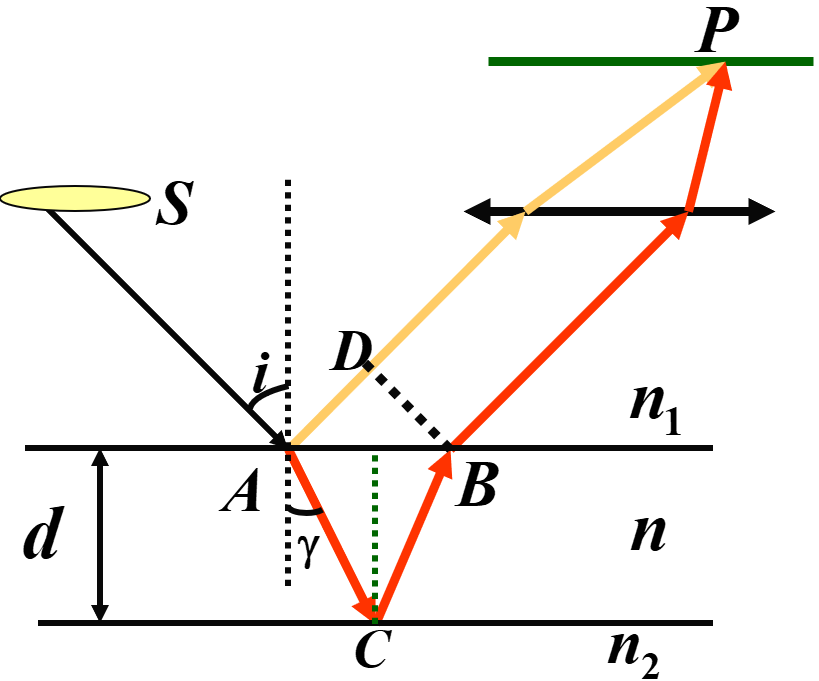
\includegraphics[width=0.4\textwidth]{15.46_1}
	\caption{Problem 15.46 voltage transfer characteristics}
\end{figure}

15.47 The saturated output voltages are $\pm V_P$ for the Schmitt trigger in Figure P15.47. (a) Derive the expressions for the crossover voltages $V_{TH}$ and  $V_{TL}$ (b) If $V_P= 12$V, $V_{REF}= - 10$V, and $R_3= 10$k$\Omega$, find $R_1$ and $R_2$ such that the switching point is $V_S=-5$ V and the hysteresis width is 0.2 V. (c) Sketch the voltage transfer characteristics.
\begin{figure}[H]
	\centering
	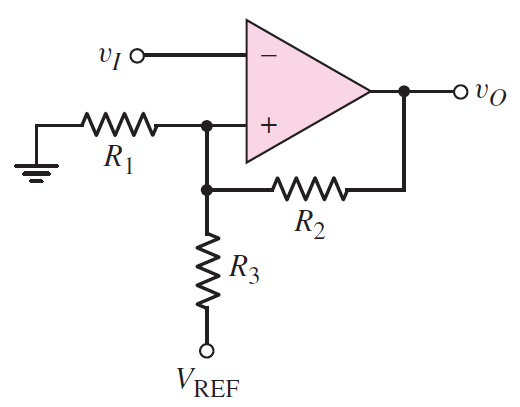
\includegraphics[width=0.4\textwidth]{15.47}
	\caption{Problem 15.47}
\end{figure}
\noindent Solution:

(a)For $V_O=V_P$:
$$
	\frac{V_O-V_{TH}}{R_2}+\frac{V_{REF}-V_{TH}}{R_3}=\frac{V_{TH}}{R_1}\Rightarrow V_{TH} =\frac{\dfrac{V_{REF}}{R_3}+\dfrac{V_P}{R_2}}{\left(\dfrac1{R_1}+\dfrac1{R_2}+\dfrac1{R_3}\right)}
$$

For $V_O=-V_P$:
$$
\frac{V_O-V_{TH}}{R_2}+\frac{V_{REF}-V_{TH}}{R_3}=\frac{V_{TH}}{R_1}\Rightarrow V_{TH} =\frac{\dfrac{V_{REF}}{R_3}-\dfrac{V_P}{R_2}}{\left(\dfrac1{R_1}+\dfrac1{R_2}+\dfrac1{R_3}\right)}
$$

(b) Equations as follow:
$$
	\left\{\begin{aligned}
		&\frac{\dfrac{V_{REF}}{R_3}}{\left(\dfrac1{R_1}+\dfrac1{R_2}+\dfrac1{R_3}\right)}=-5\\
		\Delta &V_T=V_{TH}-V_{TL}=\frac{\dfrac{2V_P}{R_2}}{\left(\dfrac1{R_1}+\dfrac1{R_2}+\dfrac1{R_3}\right)}=0.2
	\end{aligned}\right.\Rightarrow R_1=10.17\mathrm{k\Omega},R_2=600\mathrm{k\Omega}
$$

(c)$V_{TL}=-5.1\mathrm{V},V_{TH}=-4.9\mathrm{V}$
\begin{figure}[H]
	\centering
	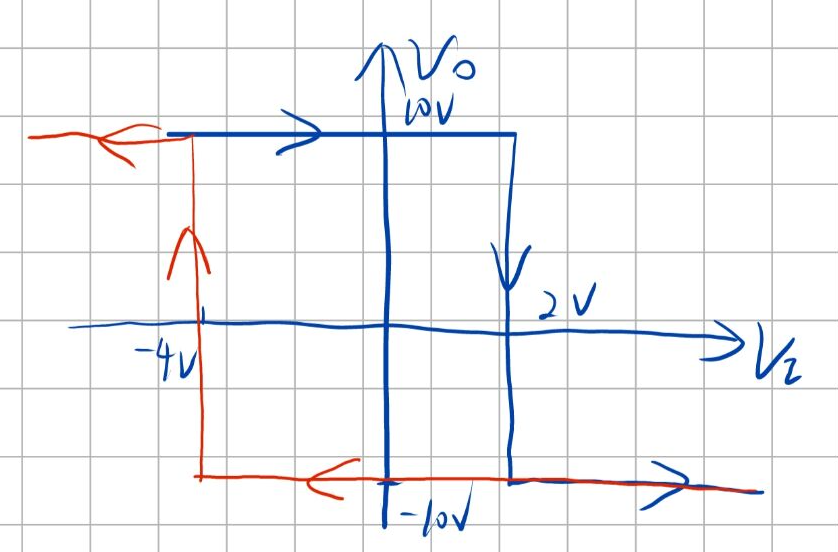
\includegraphics[width=0.4\textwidth]{15.47_1}
	\caption{Problem 15.47 voltage transfer characteristics}
\end{figure}
15.48 (a) Plot the voltage transfer characteristics of the comparator circuit in Figure P15.48 assuming the open-loop gain is infinite. Let the reverse Zener voltage be $V_{Z}=5.6$ V and the forward diode voltage be $V_{\gamma}=0.6$ V. (b) Repeat part (a) for an open-loop gain of $10^3.(c)$ Repeat part (a) for 2.5 V
applied to the inverting terminal of the comparator.
\begin{figure}[H]
	\centering
	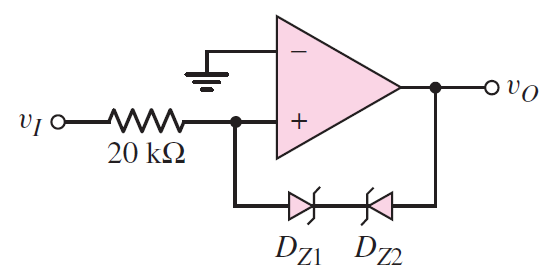
\includegraphics[width=0.4\textwidth]{15.48}
	\caption{Problem 15.48}
\end{figure}
\noindent Solution:

(a)case 1: $|V_P|<6.2$V, the Diodes are open:
\begin{figure}[H]
	\centering
	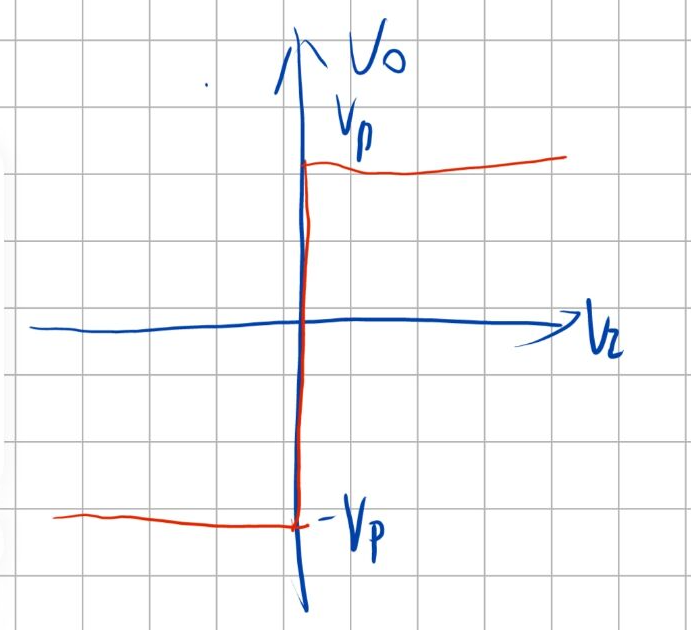
\includegraphics[width=0.4\textwidth]{15.48_1}
	\caption{Problem 15.48}
\end{figure}
case 2: $|V_P|>6.2$V, the one of the Zener Diodes work, $|V_O|=6.2$V and input can be ignored
\begin{figure}[H]
	\centering
	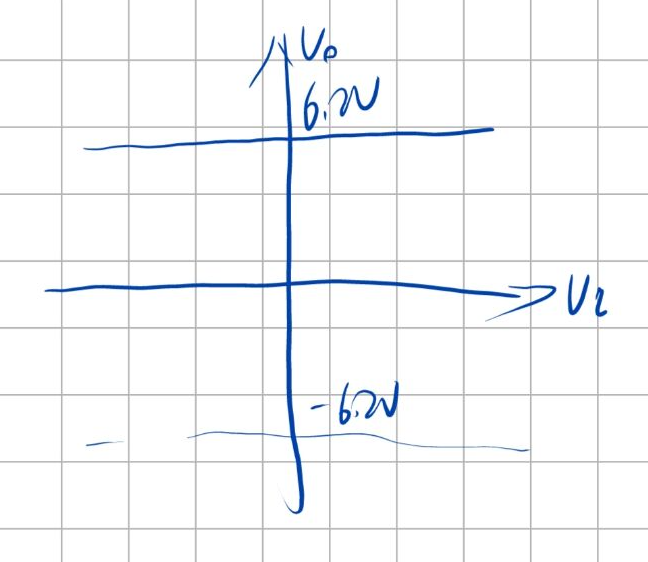
\includegraphics[width=0.4\textwidth]{15.48_2}
	\caption{Problem 15.48}
\end{figure}
(b) Same as (a)

(c)when $V_O < 8.7$ V and $V_O>$3.7 V, work as comparator. Otherwise the input has no
control

15.79 The voltage regulator shown in Figure P15.79 is a variable voltage, 0 to 5 A
power supply. The transistor parameters are $\beta=80$ and $V_{BE}( $on$) = 0.7$ V. The op-amp has a finite open-loop gain of $A_{OL}=5\times10^3$ .The zero-current Zener voltage is $V_{ZO}=5.6$ V and the Zener resistance is $r_z=12\Omega.(a)$ For $I_Z= 12$mA,find $R_1.( $b$) $ Determine the range of output voltage as the potentiometer $R_{3}$ is varied.(c) If the potentiometer is set such $x= 1$, determine $:R_o$ of the op-amp is zero.
\begin{figure}[H]
	\centering
	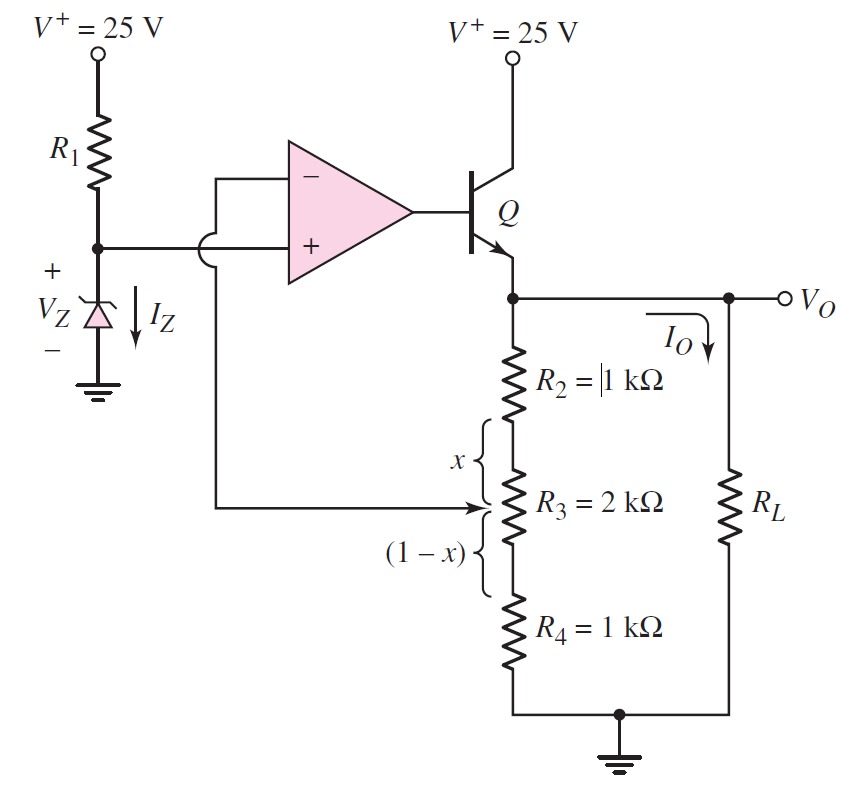
\includegraphics[width=0.4\textwidth]{15.79}
	\caption{Problem 15.79}
\end{figure}
\noindent Solution:

(a)
$$R_1+r_z=\frac{V^+}{I_Z}=\frac{25}{12}=2.0833\mathrm{k}\Omega\Rightarrow R_1=2.0713\mathrm{k}\Omega$$

(b)$V^+=V_Z+I_Z=5.744\mathrm{V}$

If $x=0$,$$V^+=\left(\frac{R_3+R_4}{R_2+R_3+R_4}\right)·V_O\Rightarrow V_O==7.659\mathrm{V}$$

If $x=1$, \\
	$$V^+ =\left({\frac{R_{4}}{R_{2}+R_{3}+R_{4}}}\right)\cdot V_{O}\Rightarrow V_{0}=22.976\mathrm{V}  \\
	 $$
	 
So $7.659 \leq V_{O}\leq22.976\mathrm{V}$

(c)???

15.80 The parameters of the transistor in Figure P15.80 are $\beta=80$ and $V_{EB}( on) = 0.6$ V.The Zener diode is ideal with $V_{\mathbb{Z}}=6.8$ V and the op-amp is ideal. (a) Determine the range of load resistance $R_L$ such that the load current is a constant. What is the value of the constant load current? (b) If the Zener diode has a resistance $r_z=20\Omega$ and the power supply is in the range $16\leq V_S\leq20$ V, determine the range in output current for 
$R_L= 5$k$\Omega.$
\begin{figure}[H]
	\centering
	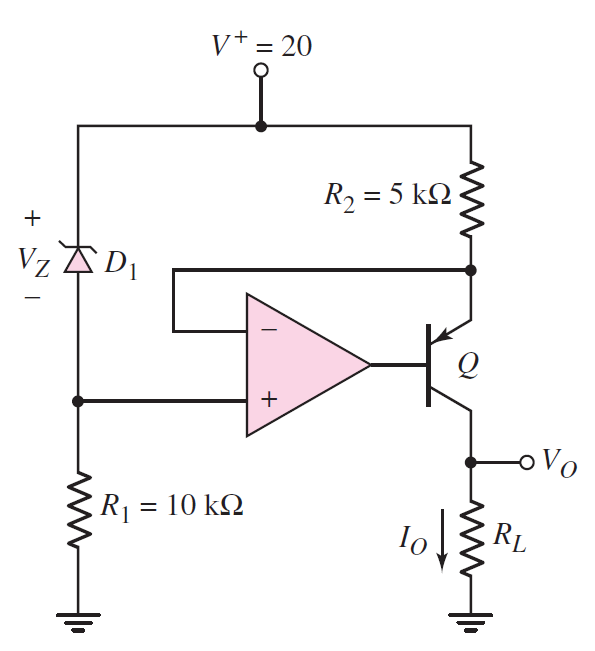
\includegraphics[width=0.4\textwidth]{15.80}
	\caption{Problem 15.80}
\end{figure}
\noindent Solution:

(a)
	$$I_{O}=\left(\frac{\beta}{1+\beta}\right)\cdot \frac{V_Z}{R_2}=1.343\mathrm{mA}$$
	$$R_L(\max)=\frac{V^+-V_Z-V_{BE}(on)}{I_O}=9.38\mathrm{k\Omega}$$
	
(b)For $V_S=16$V
$$
	I_O=\left(\frac{\beta}{1+\beta}\right)\dfrac{V_S-\dfrac{R_1}{R_1+r_Z}(V_S-V_Z)}{R_2}=1.3484\mathrm{mA}
$$

For $V_S=16$V
$$
I_O=\left(\frac{\beta}{1+\beta}\right)\dfrac{V_S-\dfrac{R_1}{R_1+r_Z}(V_S-V_Z)}{R_2}=1.3468\mathrm{mA}
$$
\end{document}